\documentclass{beamer}

\usepackage[T1]{fontenc}
\usepackage[utf8]{inputenc}
\usepackage{lmodern}
\usepackage{graphicx}
\usepackage[absolute,overlay]{textpos}
\usepackage{multicol}
\usepackage{listings}
\usepackage{svg}

%% Beamer customization--------------------------------------------------------

\usepackage{xcolor}


\usepackage{tikz}

\usetheme{Warsaw}

%% Themes
% Outer themes
\useoutertheme{shadow}
% Rounded boxes and shadows
\useinnertheme[shadow=true]{rounded}
% Solid \item symbols
\useinnertheme{circles}

%% Custom colors
\definecolor{rltgreen}{rgb}{0,0.5,0}
\definecolor{pasteur}{RGB}{0,90,154}
\setbeamerfont{block title}{size={}}
\setbeamercolor{structure}{fg=pasteur}
\setbeamercolor{item}{fg=pasteur}


%Color of title
\setbeamertemplate{frametitle}
{    \nointerlineskip
    \begin{beamercolorbox}[sep=0.3cm,ht=1.8em,wd=\paperwidth]{frametitle}
        \vbox{}\vskip-2ex%
        \strut\insertframetitle\strut
        \vskip-0.8ex%
    \end{beamercolorbox}
}
% Hide navigation symbols
\setbeamertemplate{navigation symbols}{}

%% Title block
\setbeamercolor*{title}{use=structure,fg=white,bg=pasteur}

\makeatletter

%% Top infolines
\setbeamertemplate{headline}{%
\leavevmode%
  \hbox{%
    \begin{beamercolorbox}[wd=\paperwidth,ht=2.5ex,dp=1.125ex]{palette quaternary}%
    \insertsectionnavigationhorizontal{\paperwidth}{}{\hskip0pt plus1filll}
    \end{beamercolorbox}%
  }
}


%% Define Snakemake -----------------------------------------------------------

\definecolor{eclipseBlue}{RGB}{42,0.0,255}
\definecolor{eclipseGreen}{RGB}{63,127,95}
\definecolor{eclipsePurple}{RGB}{127,0,85}

\lstset{language=Python}
\lstset{
    basicstyle=\scriptsize\ttfamily,
    morekeywords={rule, output, shell, params, run, configfile, temp, log},
    showstringspaces=false,
    commentstyle=\color{eclipseGreen}, % style of comments
    keywordstyle=\color{eclipsePurple}, % style of keywords
    stringstyle=\color{eclipseBlue}, % style of strings
}



%% Set up title ---------------------------------------------------------------

\title[Sequana]{A very brief history of Sequana}
\author[T. Cokelaer]{Thomas Cokelaer}
\institute{Institut Pasteur}
\date{Jan 24th 2017, Institut Pasteur (HUB talk)}


\AtBeginSection[]{
  \begin{frame}
  \vfill
  \centering
  \begin{beamercolorbox}[sep=8pt,center,shadow=true,rounded=true]{title}
    \usebeamerfont{title}\insertsectionhead\par%
  \end{beamercolorbox}
  \vfill
  \end{frame}
}

\begin{document}

%% Title slide ----------------------------------------------------------------

\begin{frame}[plain]
    \titlepage
    \begin{textblock*}{5cm}(4.5cm,0.3cm)
        
\includegraphics[scale=0.09]{images/Institut_Pasteur.png}
    \end{textblock*}
\end{frame}

%% Slides ---------------------------------------------------------------------


%\begin{frame}
    \frametitle{NGS at Biomics (Sean Kennedy)}

 Development driven by the Biomics Pole at Pasteur Institute, which involves
 many aspects of NGS including :

 \tiny
 \begin{block}{https://research.pasteur.fr/en/team/biomics/}
  \begin{itemize}
  \item De novo and targeted sequencing of viruses, prokaryotes and eukaryotes
  \item Variant (SNP, indel, large rearrangements) detection
  \item Transcriptional analysis (RNA-Seq) for both prokaryotes and eukaryotes
  \item 16S and deep-sequencing metagenomic studies (mouse, human, and other
environments)
  \item Epigenetics (CHIP-Seq, methylation studies)
  \end{itemize}
 \end{block}
 \small
\end{frame}

%\begin{frame}
 \frametitle{Needs}

    \begin{block}{What do we have \dots or not ?}
     
\includegraphics[scale=0.05]{../../images/positive.png}\; A bunch of pipelines dedicated
to NGS data\\
     
\includegraphics[scale=0.05]{../../images/positive.png}\; Expertise\\
     
\includegraphics[scale=0.05]{../../images/negative.png}\; Lack of \\
    \begin{itemize}
     \item traceability ?
     \item reproducibility ?
     \item co-development ?
     \item common framework ?
    \end{itemize}
    \end{block}

    \begin{block}{What do we need ?}
    \begin{itemize}
     \item A framework to combine or re-use existing pipelines
     \item Fast development (iterative process)
     \item Continuous Integration and Quality Software (reproducibility, 
           traceability, test, documentation)
    \end{itemize}
    \end{block}
\end{frame}


\begin{frame}
    \frametitle{Why Sequana ?}


    \begin{block}{Provide a toolbox to parse and analyse NGS data sets }
    \begin{itemize}
        \item Simplified version to external dependencies
        \item Include pandas for data mining
        \item Matplotlib for visualisation
    \end{itemize}
    \end{block}

    \begin{block}{Enforce a common framework}
    \begin{itemize}
        \item Using Snakemake as a common language to design new pipelines
        \item Provide reusable snakemake rules and modules
    \end{itemize}
     \end{block}

    \begin{block}{An entry point to a high quality software}
    \begin{itemize}
        \item Quality (doc + tests)
        \item Diffusion
        \item Reproducibility
    \end{itemize}
    \end{block}

\end{frame}







\section{Sequana: a Python library}

\begin{frame}
\frametitle{Python behind the scene}
 \begin{block}{Python as a glue language}
     - Make use of anaconda for installation and various dependendies. \\
     - For low-level computations, use existing libraries (e.g., pysam)
 \end{block}
 
 \begin{block}{Dev of original tools}
  e.g. coverage or quick taxonomy (see talk on sequana\_coverage)
 \end{block}
 
 \begin{block}{add missing bricks}
  - kraken2krona
  - ...
 \end{block}

 \begin{block}{HTML Reporting}
  Based on Jinja and Sequana reports.
 \end{block}
\end{frame}



\section{Sequana: snakemake as a workflow manager}


\begin{frame}
 
\includegraphics[width=1.\textwidth, height=0.8\textheight]{images/julia_nice.png}
\end{frame}


\begin{frame}[fragile]
\frametitle{Snakemake workflow = Snakefile + config file}
\begin{block}{pseudo working example of a simple workflow:}
  \begin{lstlisting}
configfile: "fractal.yaml"
config = config['fractal']
N = config['N']

rule all:
    input:expand("julia_{index}.png", index=range(N))

rule image:
    output: image="julia_{index}.png"
    run:
        xy = "%.3f +%.3f j" % (random(), random())
        cmd = "python -m fractal julia %s" % xy
        cmd += " --size=%(size)s --depth=%(depth)s "
        cmd += " -o julia_%s.png" % wildcards.index        
        shell(cmd % config)
\end{lstlisting} 
\end{block}
\end{frame}

\begin{frame}[fragile]
\begin{block}{configuration file}
 \begin{lstlisting}
##########################################################
# Input parameters for the fractal analysis
#
# :Parameters: 
#
# - size: output image size formatted as NxM where N and M 
#         are integers
# - depth: a integer (e.g. 200)
# - zoom: a positive value e.g. 0.5
# - N: number of random sets
fractal:
    - size: 200x200
    - depth: 200
    - zoom: 0.7
    - N: 20
 \end{lstlisting}
\end{block}
\end{frame}


\begin{frame}[fragile]

\begin{lstlisting}[basicstyle=\ttfamily\large]
snakemake -s fractal.rules 
          --configfile fractal.yaml
 \end{lstlisting}
 
\pause 
 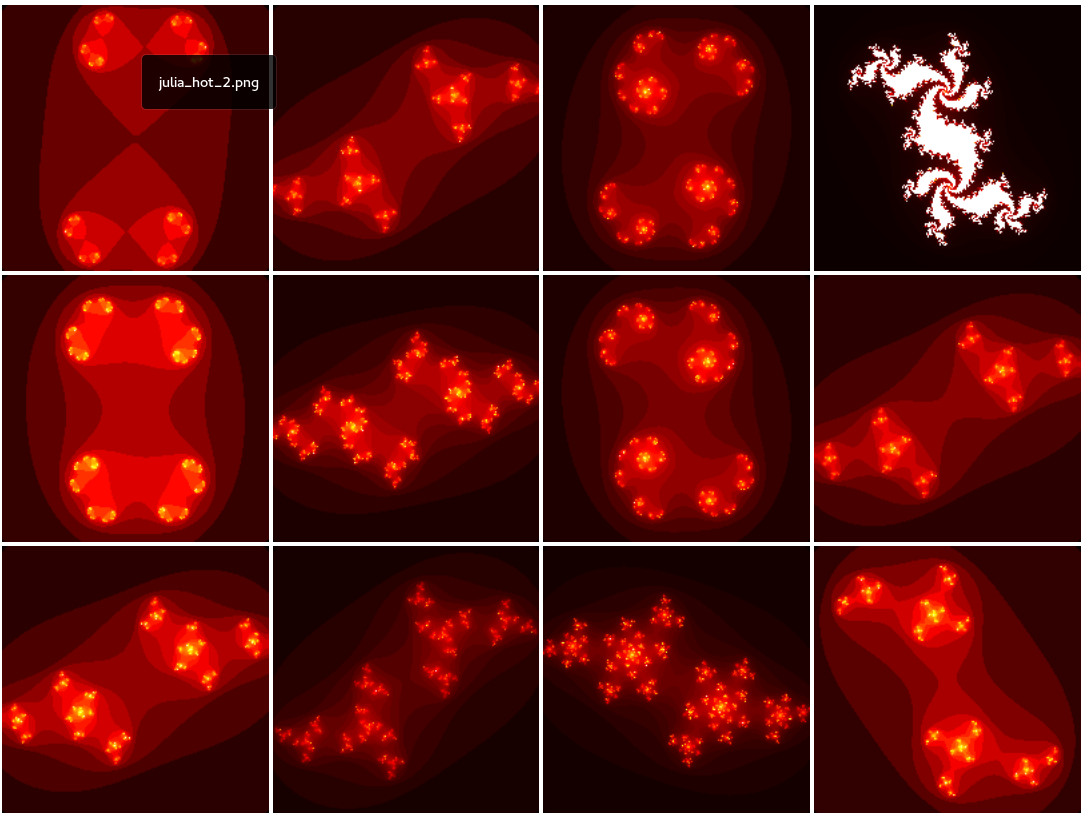
\includegraphics[scale=0.25]{./images/julia_set.png}
%sequanix -w . -s fractal.rules  -c fractal.yaml 
\end{frame}


\begin{frame}{Pipelines available in Sequana}
    \begin{textblock*}{5cm}(0.3cm,1.3cm)
        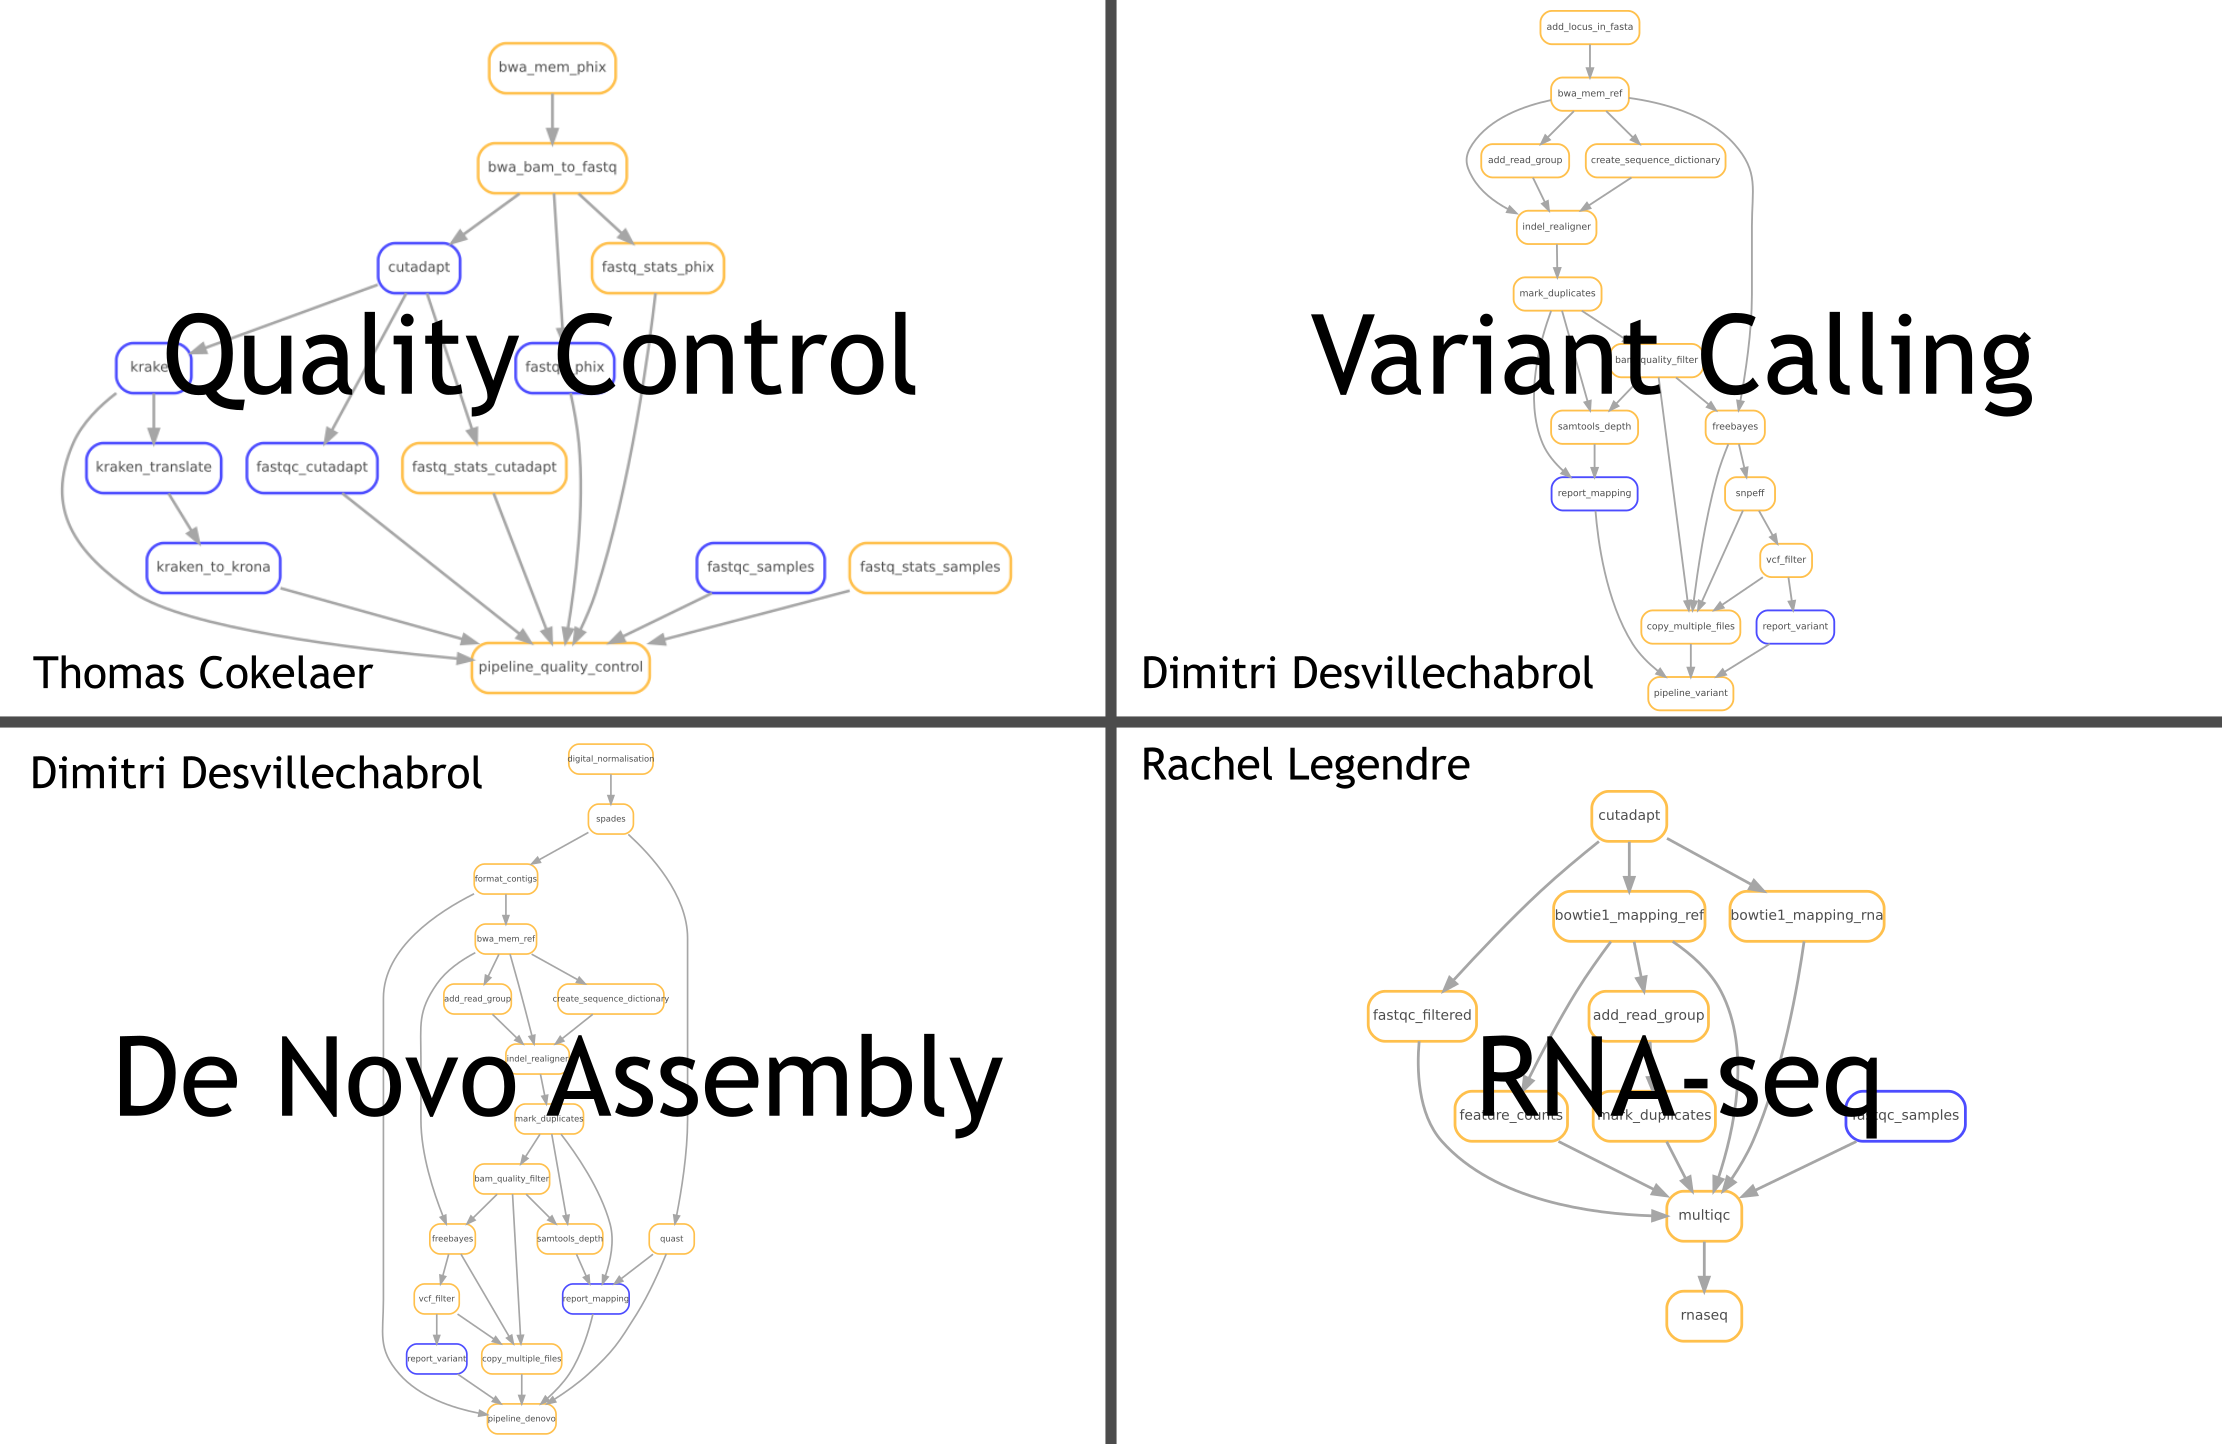
\includegraphics[scale=0.215]{images/pipelines}
    \end{textblock*}
\end{frame}





\section{Sequana: for end users with Sequanix}
\begin{frame}{GUI to simplify the usage of snakemake}
    \begin{columns}
        \begin{column}{0.5\textwidth}

            \only<1>{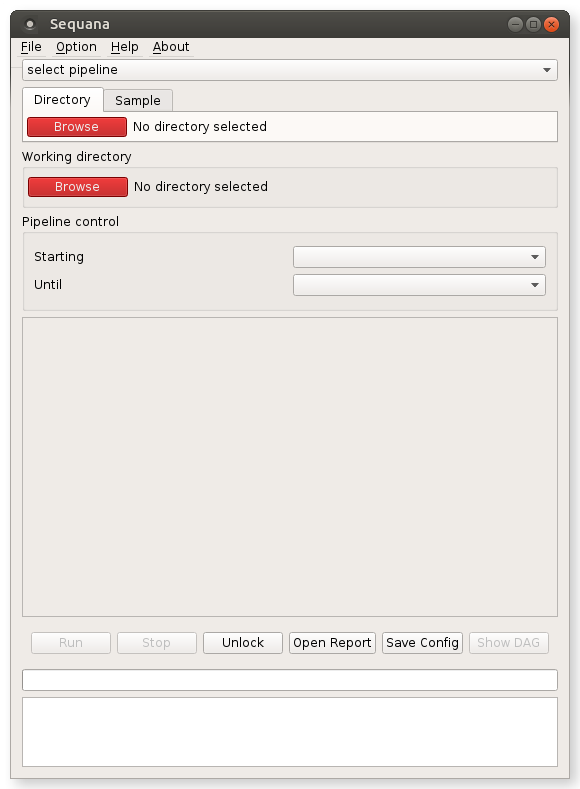
\includegraphics[scale=0.25]{../../images/sequana_init}}

            \only<2>{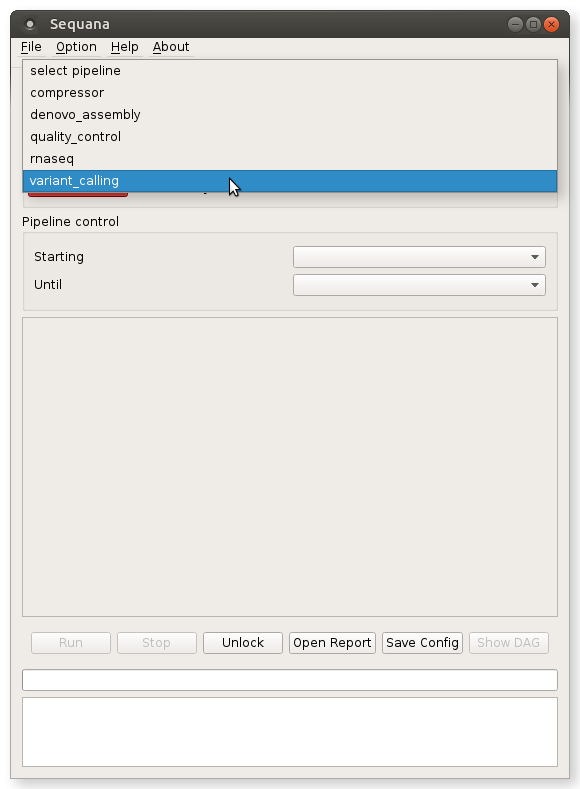
\includegraphics[scale=0.25]{../../images/choose_pipeline}}

            \only<3>{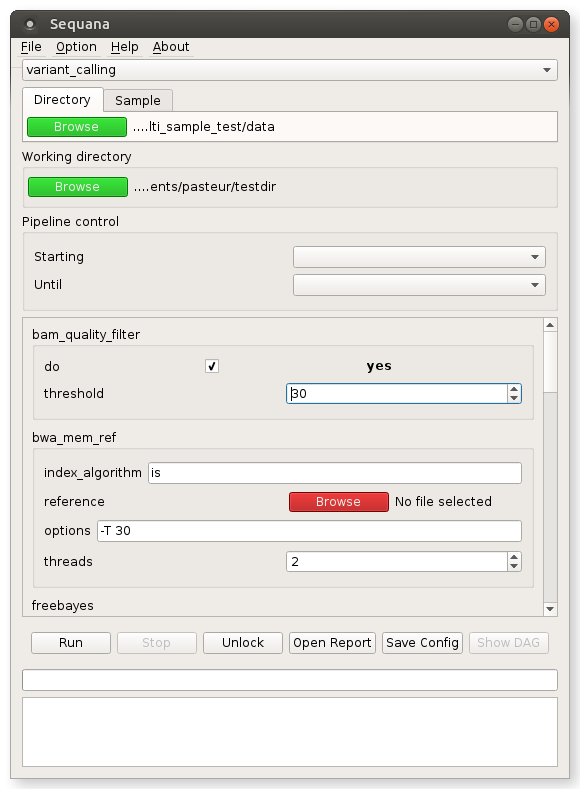
\includegraphics[scale=0.25]{../../images/choose_input_output}}

            \only<4>{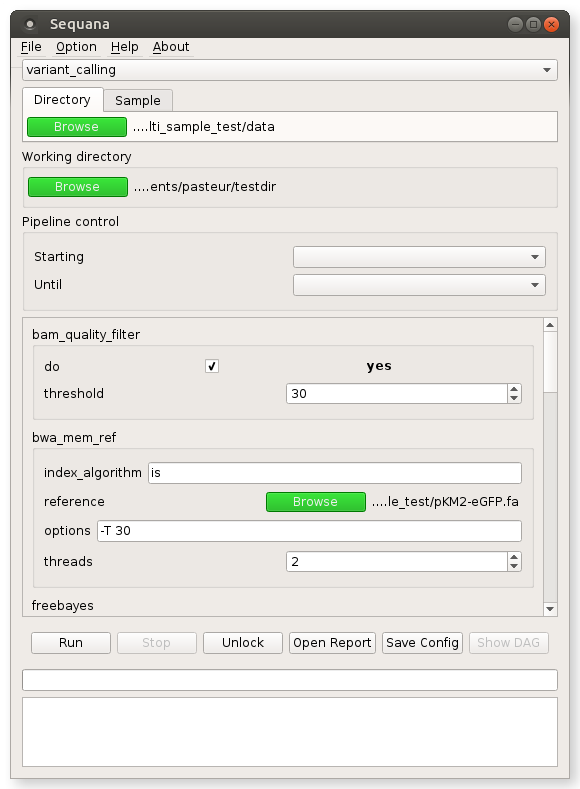
\includegraphics[scale=0.25]{../../images/sequana_pipeline}}

            \only<5>{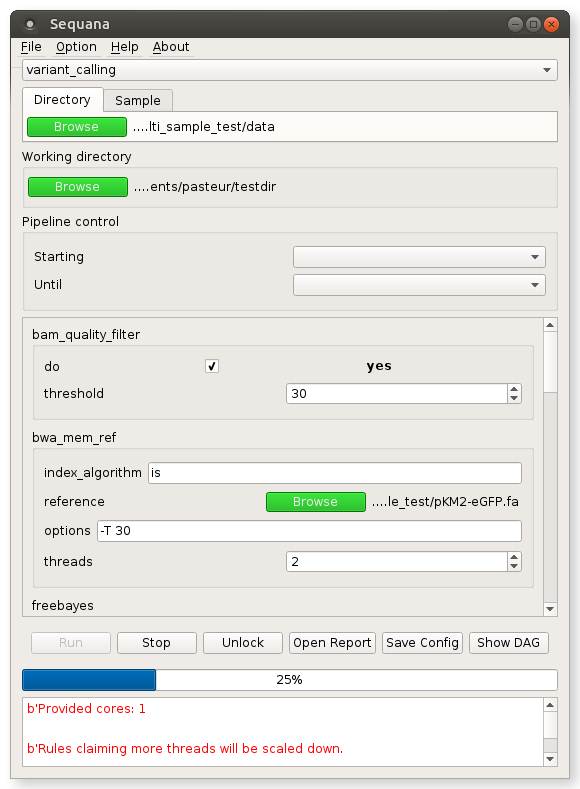
\includegraphics[scale=0.25]{../../images/sequana_running}}

            \only<6>{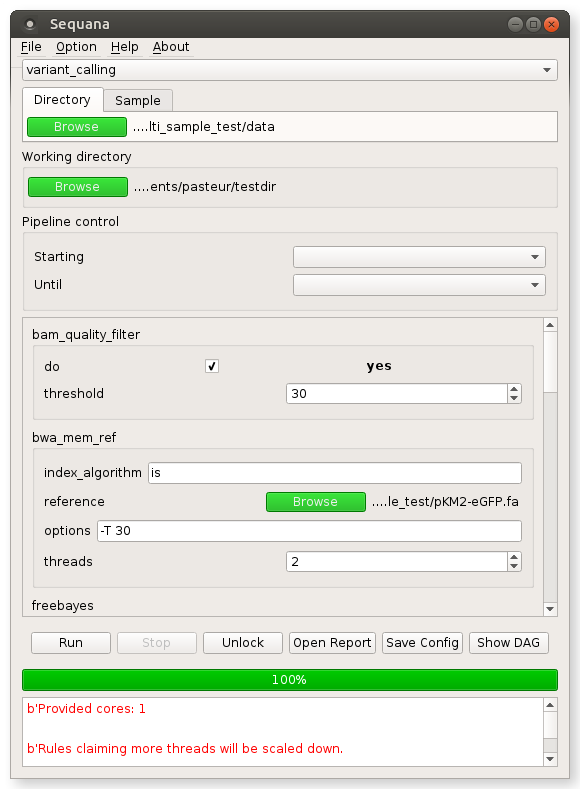
\includegraphics[scale=0.25]{../../images/sequana_finish}}

        \end{column}
        \begin{column}{0.5\textwidth}
            \only<1>{
                \begin{itemize}
                    \item Interface developed with PyQT5 and python
                    \item Wrap our snakemake pipelines to ease the usage
                    \item Usable on our cluster, which allows X11
                \end{itemize}
            }
            \only<2-6>{
            \begin{enumerate}
                \item<2-6> Choose a pipeline
                \item<3-6> Set input and output
                \item<4-6> Fill the config formular
                \item<5-6> Run the pipeline
                \item<6> Finished !
            \end{enumerate}
            }
        \end{column}
    \end{columns}
\end{frame}


 

\section{Sequana: Continuous integration}

\begin{frame}{Versioning, Test and Documentation}
\begin{tabular}{cp{8cm}}
\vspace{0.5cm}

\includegraphics[width=0.2\textwidth,height=0.1\textheight]{../../images/logo_github.png}
& https://github.com/sequana/sequana\\

\vspace{0.5cm}

\includegraphics[width=0.2\textwidth]{../../images/logo_travis.png}&  
Continuous Integration on Travis with 100 tests with 75\% coverage\\

\vspace{0.5cm}

\includegraphics[width=0.2\textwidth]{../../images/logo_sphinx.png}& 
Uses Sphinx (RST syntax) to document the source 
code and provides user guide.\\

\vspace{0.5cm}

\includegraphics[width=0.2\textwidth]{../../images/logo_rtd.png}& 
Updated after each commits on sequana.readthedocs.io
\end{tabular}

\end{frame}


\section{Summary}

\begin{frame}
 \frametitle{Summary}
Sequana is a versatile tool that provides

\begin{enumerate}
 \item A set of snakemake workflows dedicated to NGS 
 \item A GUI to execute them easily with Sequanix
 \item A Python library dedicated to NGS analysis (e.g., tools to visualise standard NGS formats).
 \item HTML reports
 \item Standalone applications:
 \begin{itemize}
    \item \textbf{sequana\_coverage} ease the extraction of genomic regions of interest and genome coverage information
    \item \textbf{sequana\_taxonomy} get a quick overview of read contents
    \item \dots
 \end{itemize}
\end{enumerate}
\end{frame}

\begin{frame}{Sequana history}
    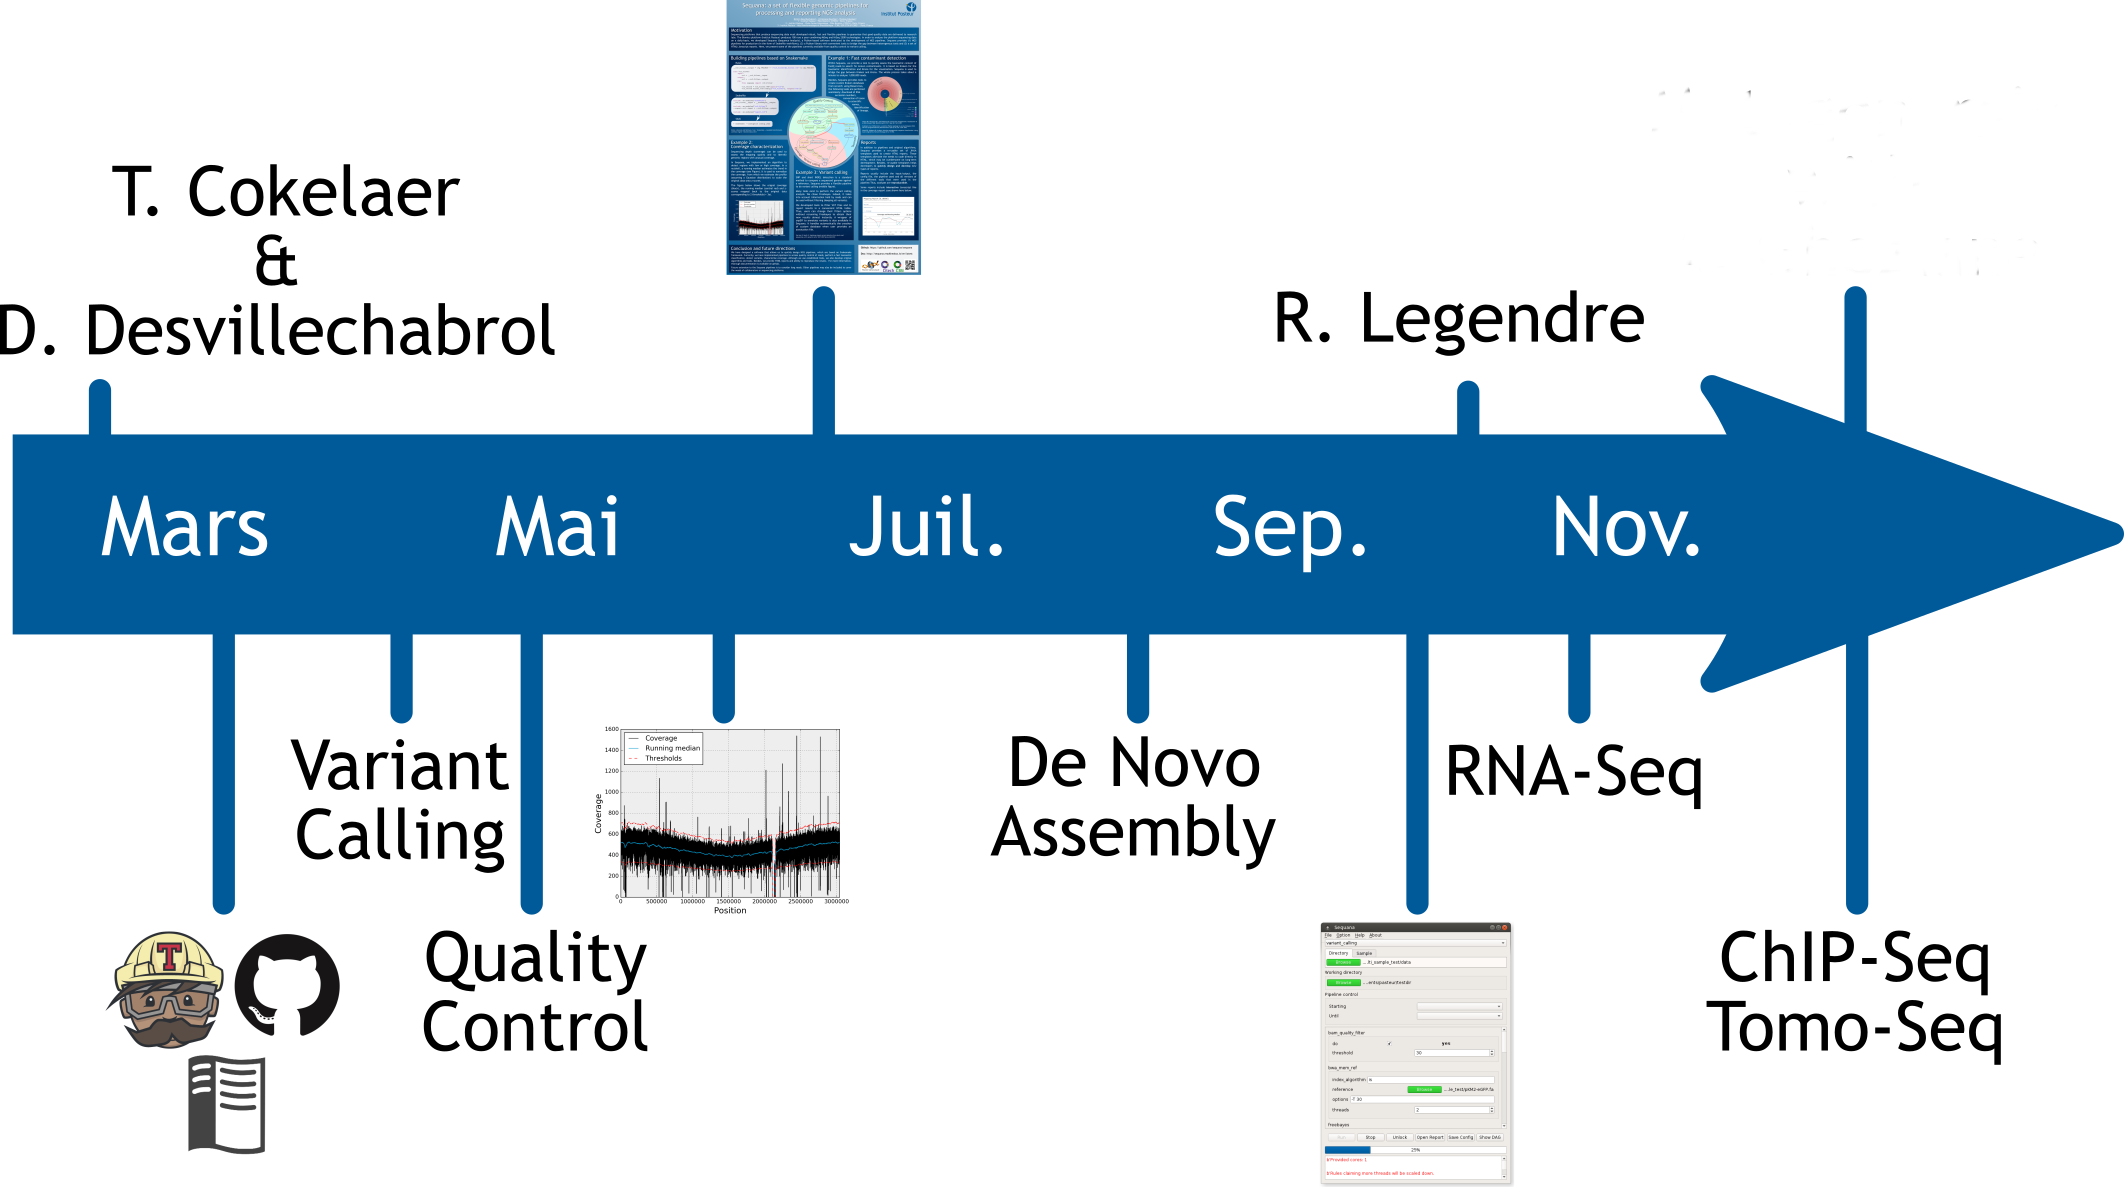
\includegraphics[scale=0.2]{images/timeline}
    \footnotetext[1]{\tiny Detection and characterization of low and high genome coverage regions using an efficient running median and a double threshold approach.
Dimitri Desvillechabrol, Christiane Bouchier, Sean Kennedy, Thomas Cokelaer
bioRxiv 092478; doi: http://dx.doi.org/10.1101/092478}
\end{frame}



\end{document}
